%!TEX TS-program = xelatex
%!TEX encoding = UTF-8 Unicode

% MICHAEL ELLIOT KING - CAD PORTFOLIO

% HEADER
	\documentclass[12pt, landscape]{article}
	\usepackage{geometry} 
	\geometry{letterpaper, textwidth=8.5in, textheight=6in}

	\usepackage{fontspec} %OpenType fonts
	\usepackage[bookmarks, colorlinks, breaklinks, 
	pdftitle={3D Printing Portfolio - Michael Elliot King}, %title of the document
	pdfauthor={Michael Elliot King}] %author of the document
	{hyperref}
	\usepackage[usenames, dvipsnames]{xcolor} % colors
	\hypersetup{linkcolor=CadetBlue,citecolor=black,filecolor=black,urlcolor=CadetBlue} % Link colors
	\usepackage{xunicode} % Allows generation of unicode characters from accented glyphs
	\defaultfontfeatures{Mapping=tex-text} % Converts LaTeX specials (``quotes'' --- dashes etc.) to unicode
	\setromanfont [Ligatures={Common}, Variant=01,]{Linux Libertine} % Main text font 

	\usepackage{setspace} %line spacing
	\linespread{1.4} %double space
	\setcounter{secnumdepth}{0} % sections are level 1 - i.e. no numbering but still in ToC

	\usepackage{pdflscape} %landscape
	\usepackage{pgfgantt} %gantt chart
	\usepackage[nottoc]{tocbibind} %adds bibliography to TOC, removes Contents fron TOC
	\usepackage{graphicx}
	\usepackage{amssymb}
	\usepackage{epstopdf}
	\DeclareGraphicsRule{.tif}{png}{.png}{`convert #1 `dirname #1`/`basename #1 .tif`.png}
	\usepackage{amsmath}
	\usepackage{mathtools}
	\usepackage{lipsum} % garbage text
	\usepackage{listings} % insert code
	\usepackage{fancyhdr} % headers and footers
	\usepackage{float} % allows putting figures exacting where in code

\title{Michael Elliot King\\[10pt]
\Huge 3D Printing Portfolio}
\normalfont \author{406 East 9th Street\\ New York, NY 10009\\[20pt]
(617)~633-0828\\
\href{mailto:mk@michaelelliotking.com}{mk@michaelelliotking.com}\\
%\href{http://www.linkedin.com/in/michaelelliotking}{linkedin.com/in/michaelelliotking}\\
\href{http://www.michaelelliotking.com}{www.michaelelliotking.com}
}

%\date{\small Last updated \today}
\date{} 

%**************************************************************************

\begin{document}
\begin{titlepage}
\linespread{1}\maketitle
\thispagestyle{empty}
\end{titlepage}

%\linespread{1.3}
%\tableofcontents
%\thispagestyle{empty}
%\clearpage

\pagestyle{fancy}
\lfoot{\small Michael Elliot King - 3D Printing Portfolio}
\rfoot{\small \href{http://www.michaelelliotking.com}{www.michaelelliotking.com}}

% AUV
	\section{Autonomous Underwater Vehicle Components}
		\paragraph{Project:} Autonomous Underwater Vehicle for the \href{http://www.mcgillrobotics.com}{McGill Robotics Design Team}
		\paragraph{Goal:} Design, manufacture, implement and test an Autonomous Underwater Vehicle to compete in the \href{http://www.robosub.org}{AUVSI Robosub Competition} in San Diego, CA.
		\paragraph{Description:} Select components on the vehicle were chosen to be printed, due to their unique shapes and small load requirements.  These parts include two marker dropper mechanisms, two torpedo launchers, two pairs of grabbing claws, two rail sliders, four projectiles, and one kill switch.  These parts were printed on a combination of Stratasys Fortus 360, Makerbot Replicator 2X, and Formlabs Form1 printers.

	\begin{figure}[H]
		\centering
		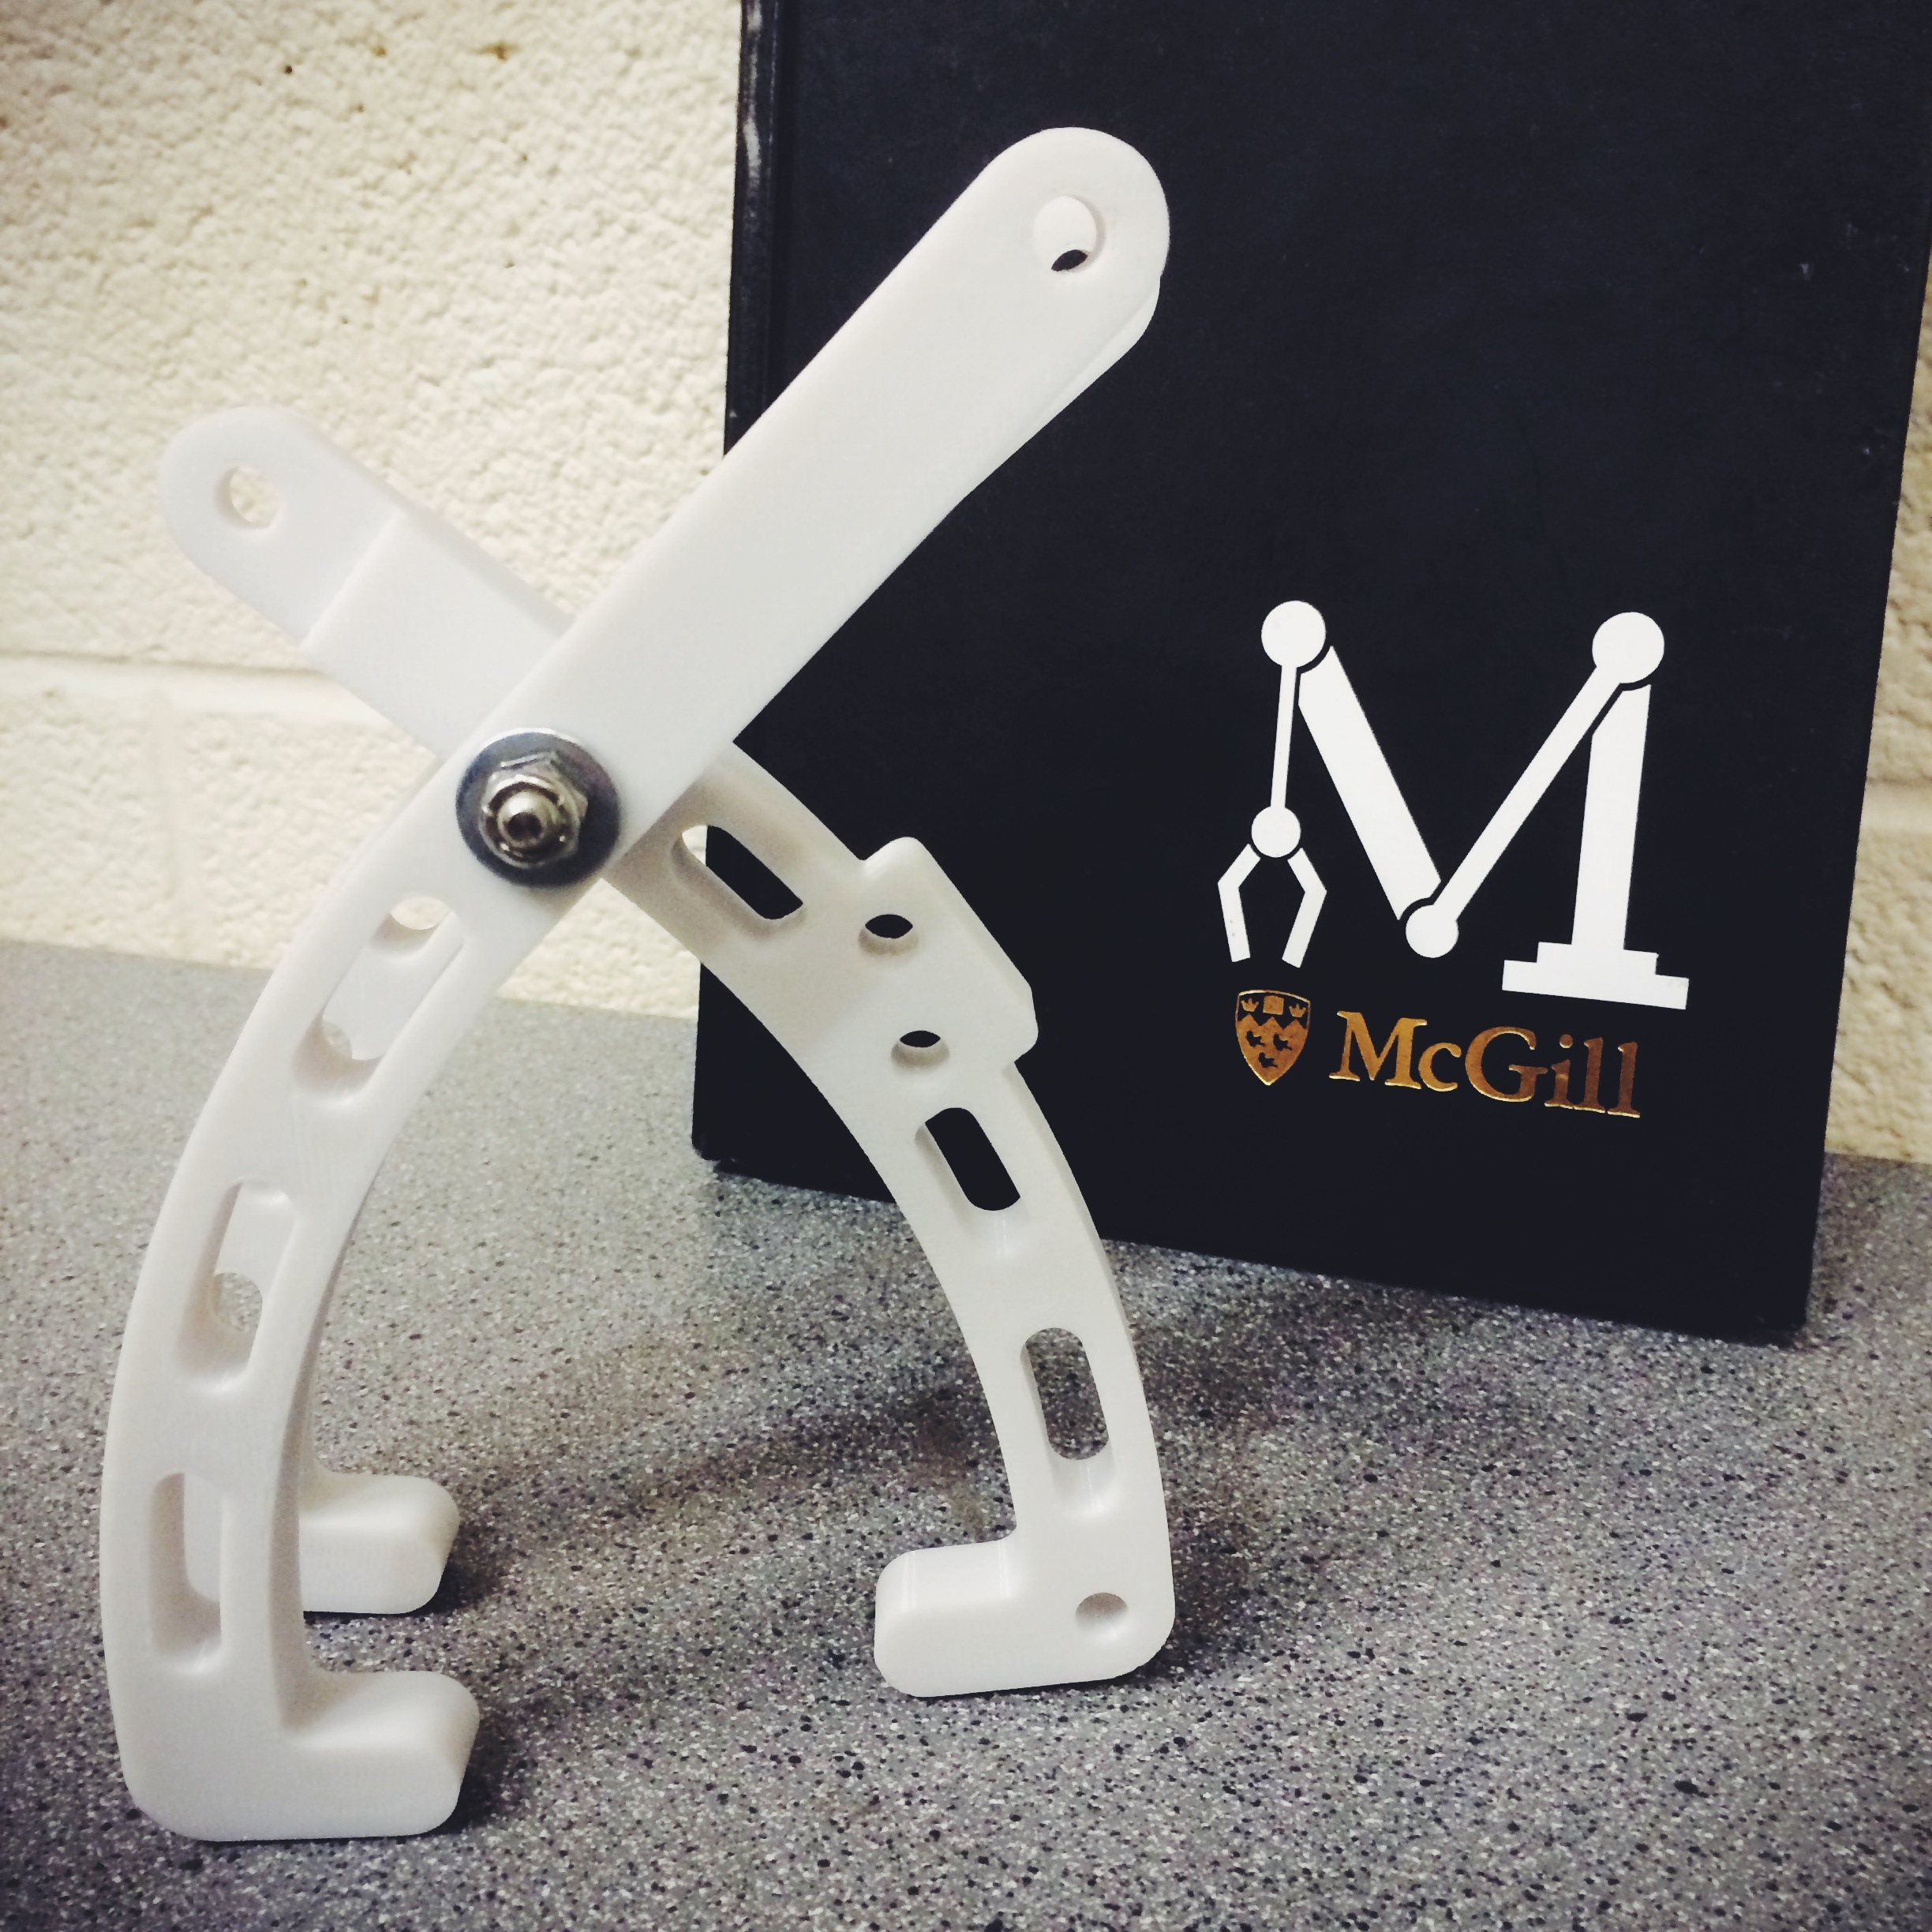
\includegraphics[height=4in]{media/grabber}
		\caption{Pneumatic claw device for picking up objects underwater}
		\label{grabber}
	\end{figure}

	The pneumatic claw uses a double-acting piston to open and close two ``fingers'' of the claw, which were printed out of ABS in a Stratasys Fortus 360 printer.  A lever on one of the fingers senses when an object has successfully been picked up using a custom, waterproof limit switch.  

	\begin{figure}[H]
		\centering
		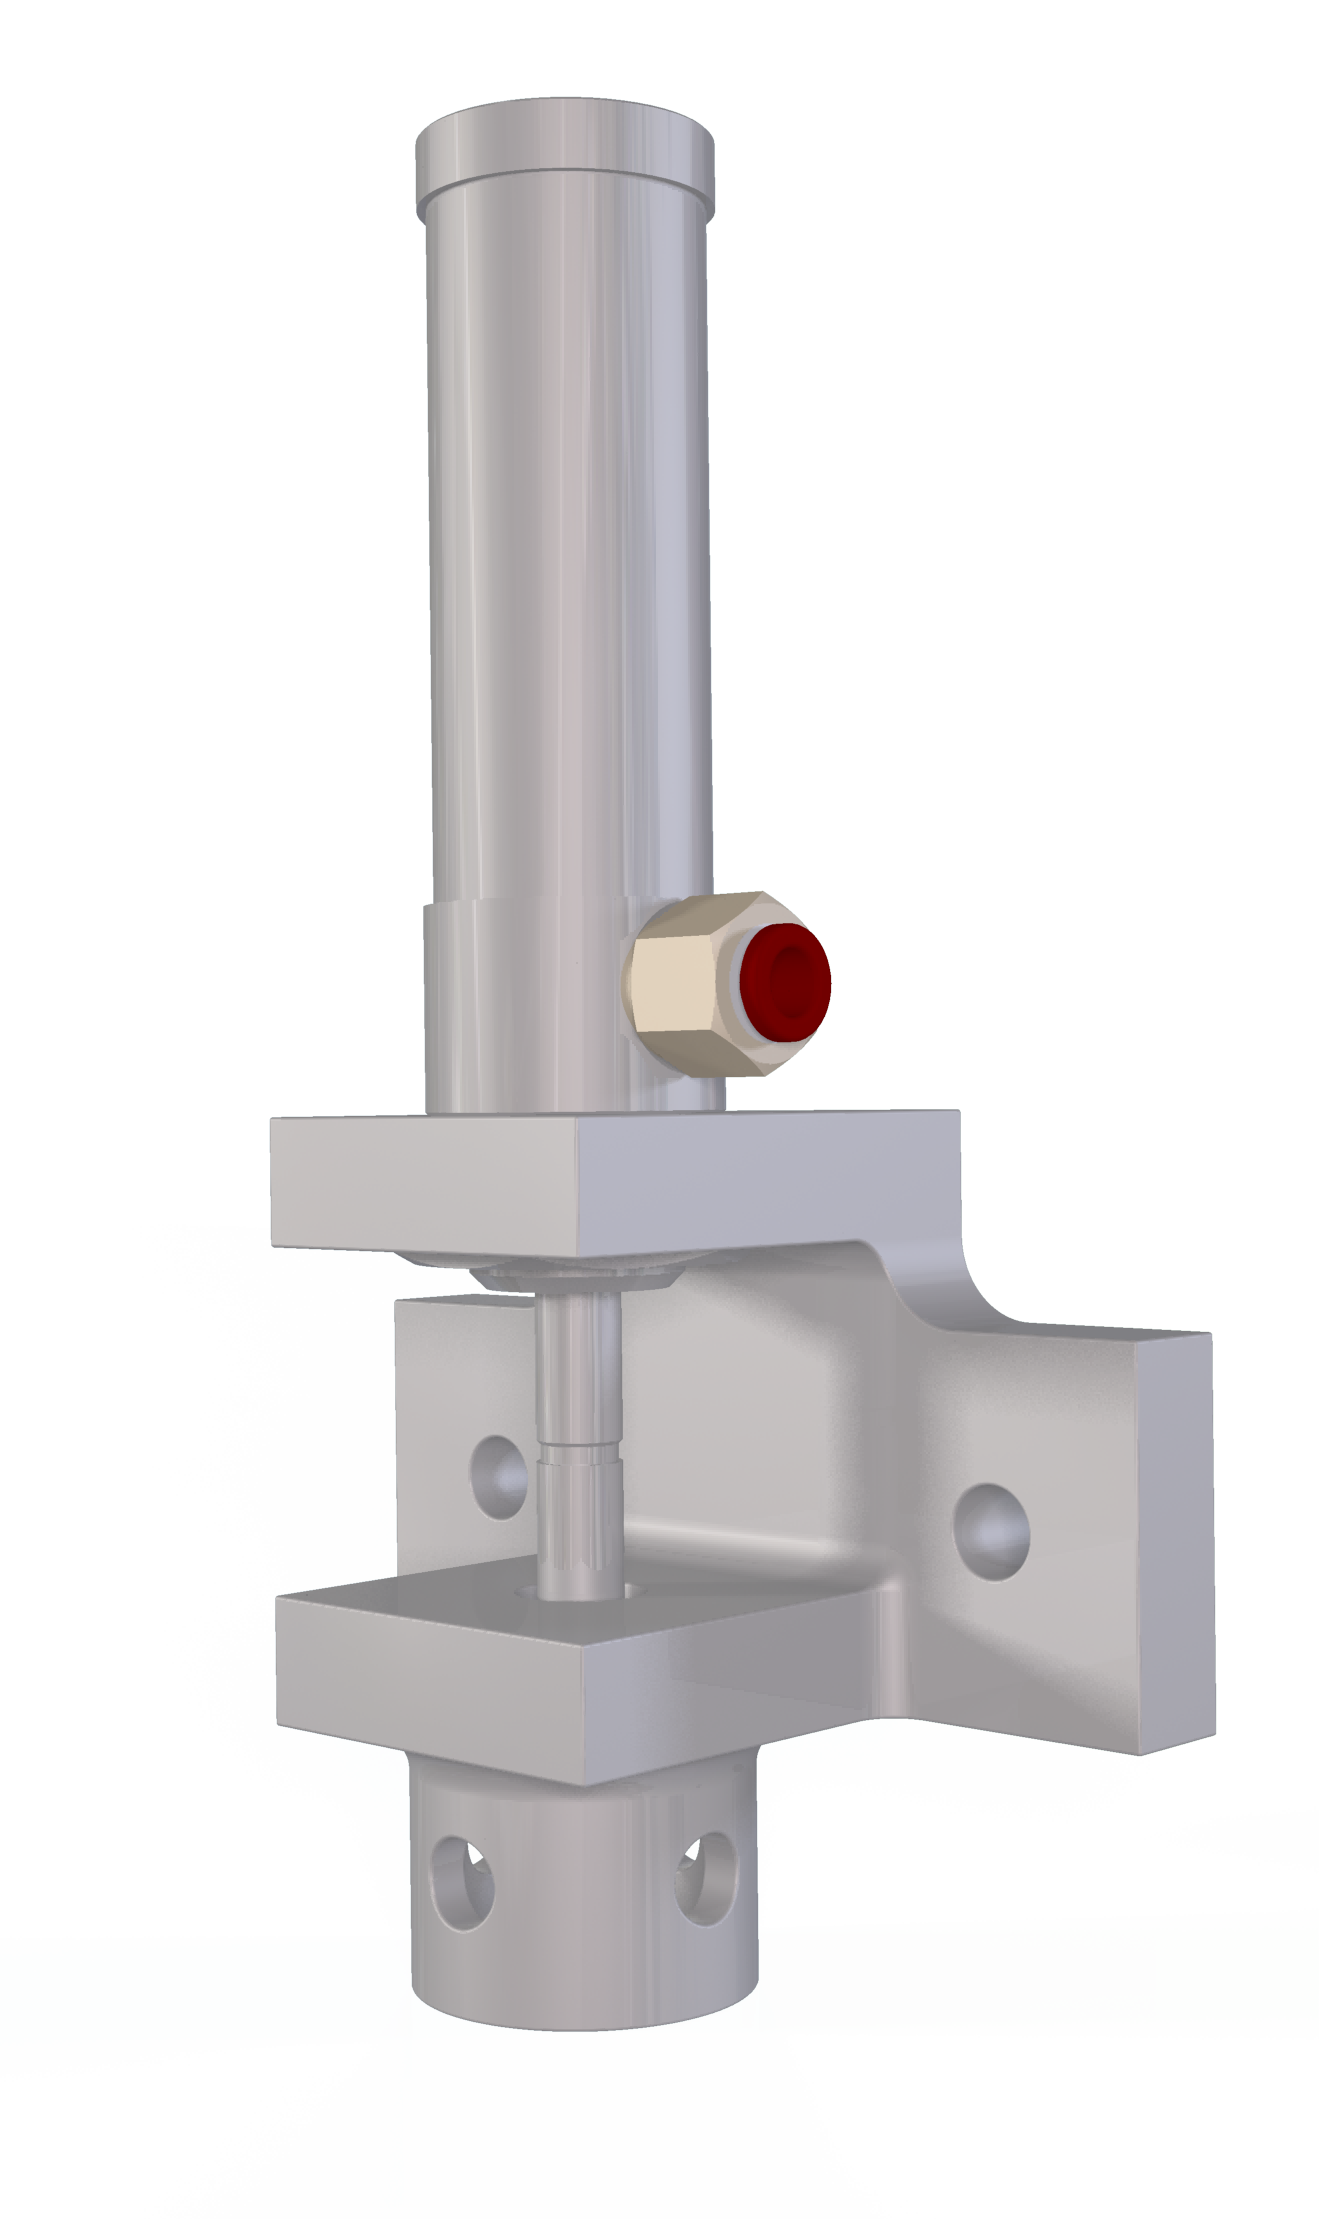
\includegraphics[height=4in]{media/marker_dropper.png}
		\caption{Pneumatic marker dropper device}
		\label{marker}
	\end{figure}

	The pneumatic marker dropper uses a reverse-acting piston with a magnet to release a ball bearing marker when over a target.  It was printed out of one piece in a FormLabs Form 1 3D printer to accommodate the piston nut, ball bearing socket, and frame-mounting points.

	\begin{figure}[H]
		\centering
		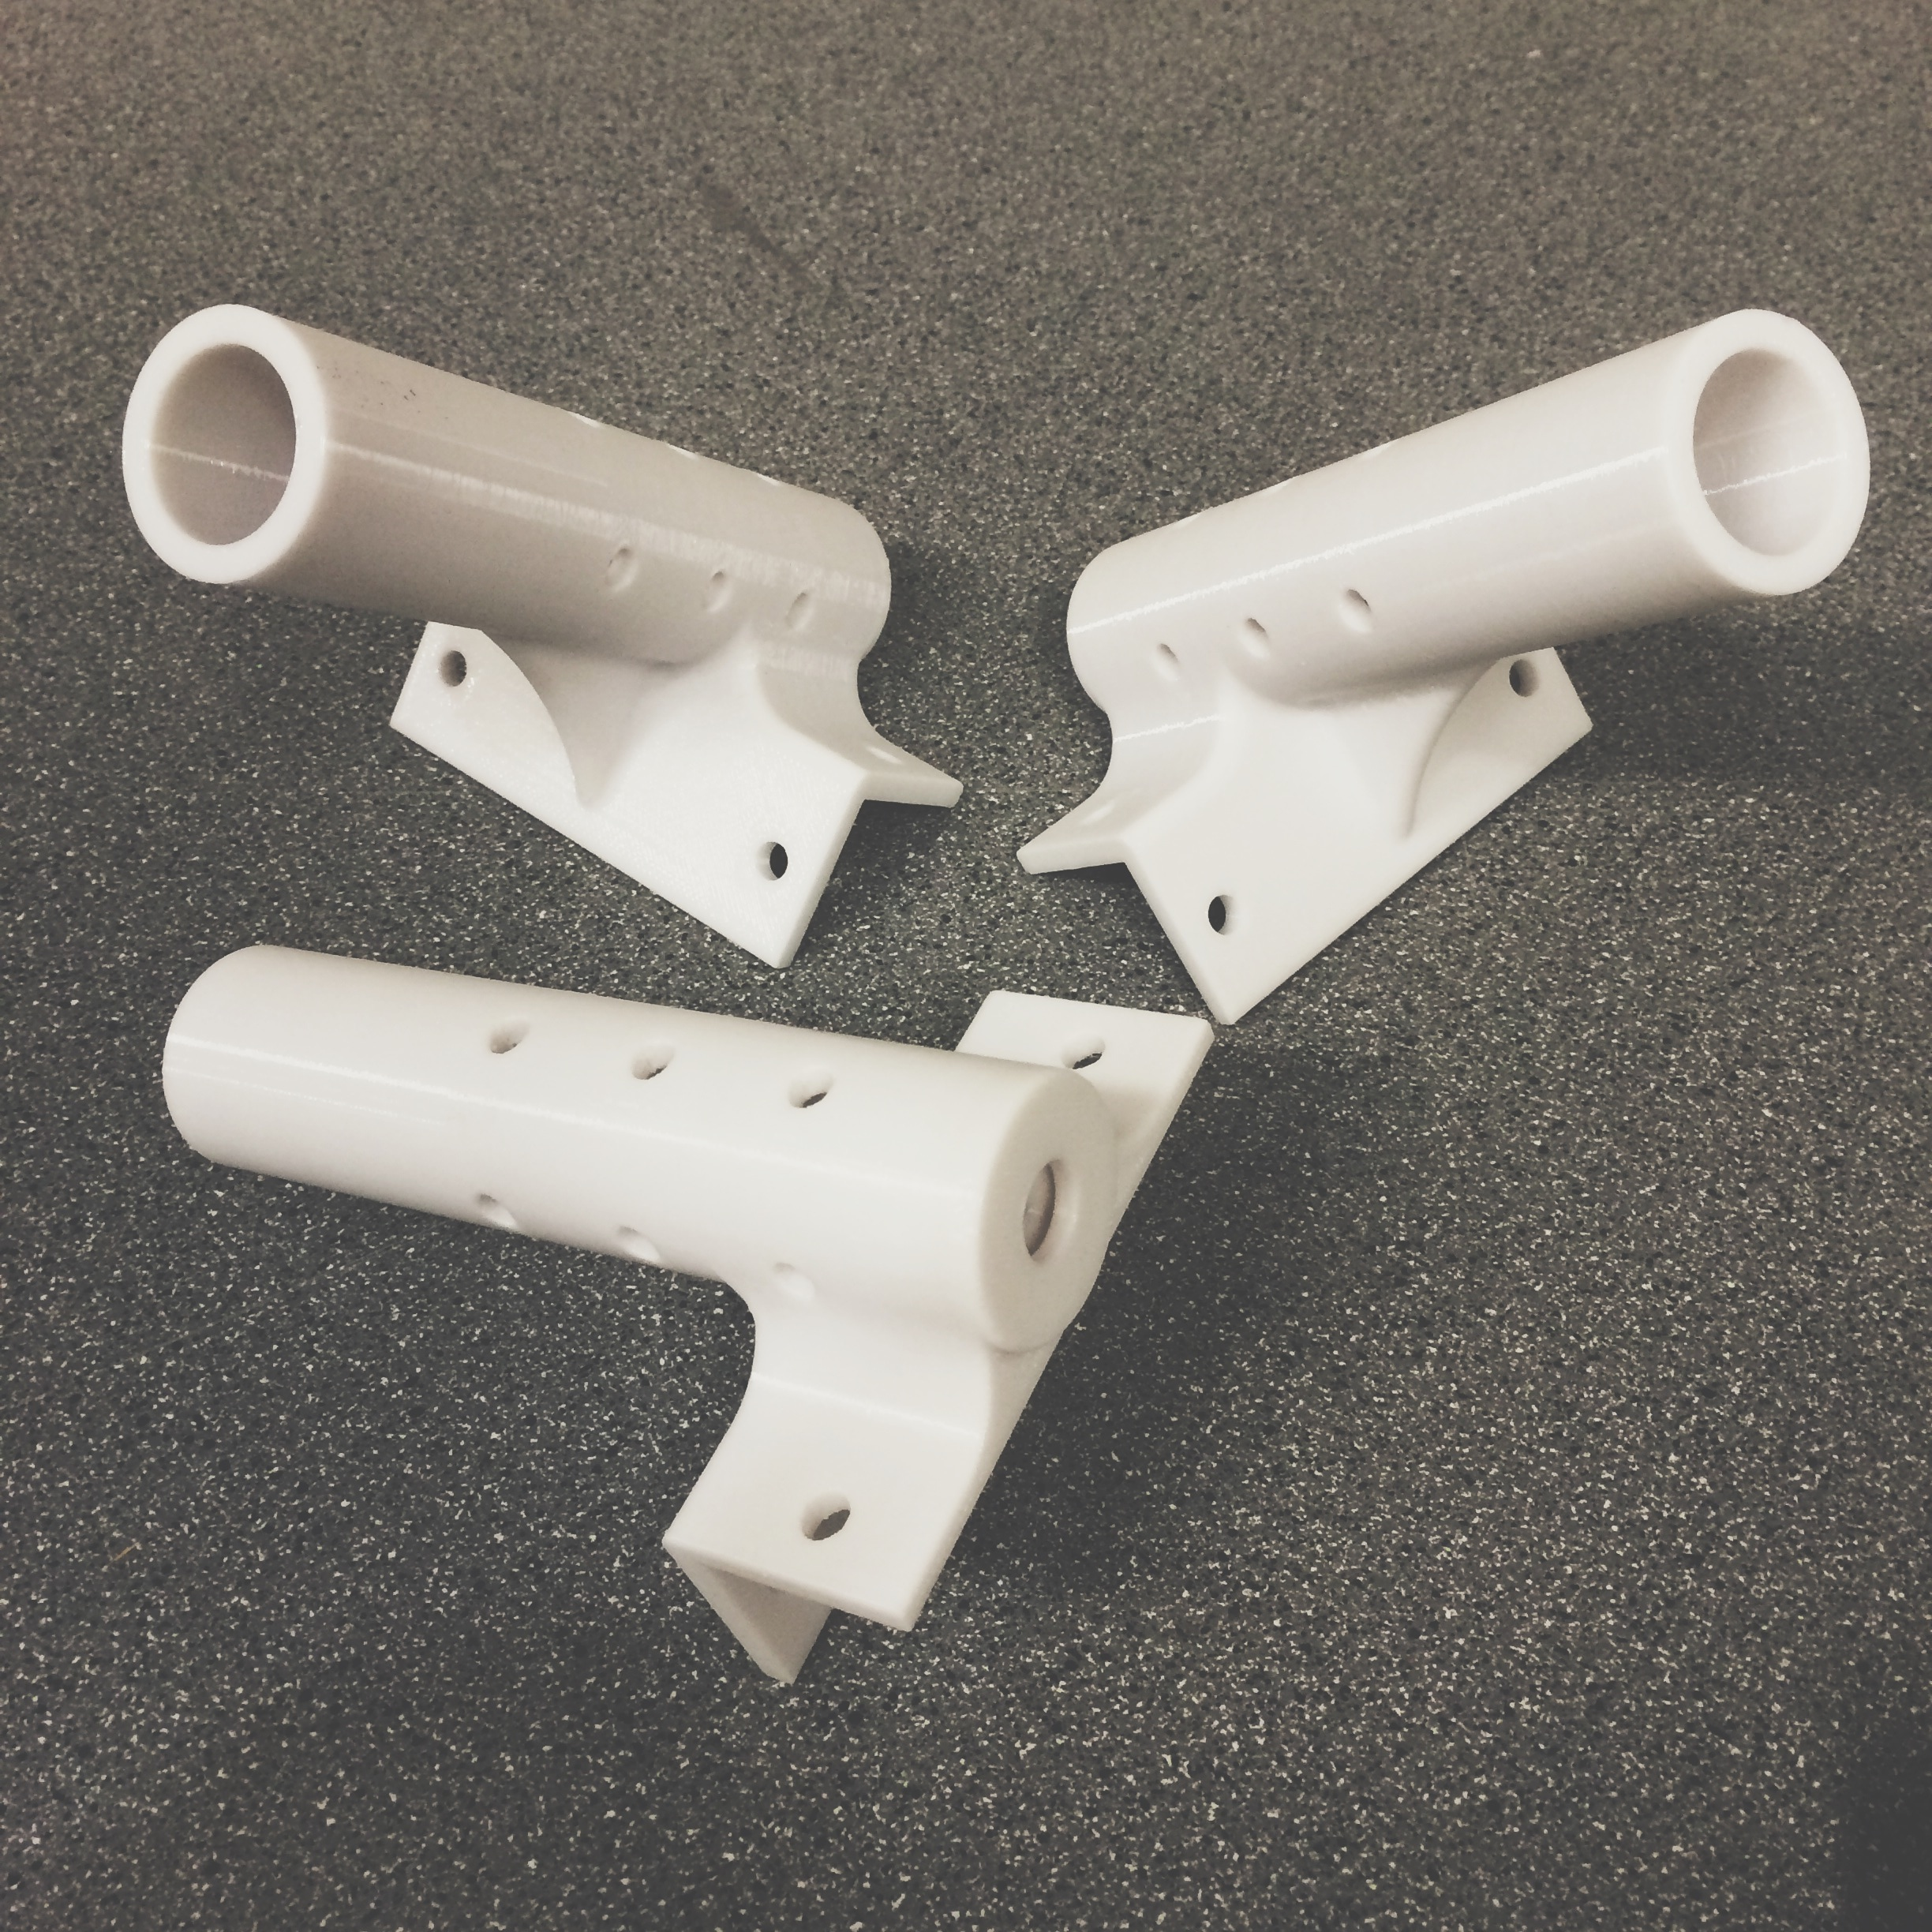
\includegraphics[height=4in]{media/launchers}
		\caption{Pneumatic torpedo launchers}
		\label{launcher}
	\end{figure}

	The torpedo launcher uses a pneumatic piston to fire a custom, 3D-printed projectile at a target at a distance of up to 5 meters.  It is printed in one piece on a Stratasys Fortus 360 printer to accommodate the piston nut, the projectile barrel, and the frame-mounting points.

	\begin{figure}[H]
		\centering
		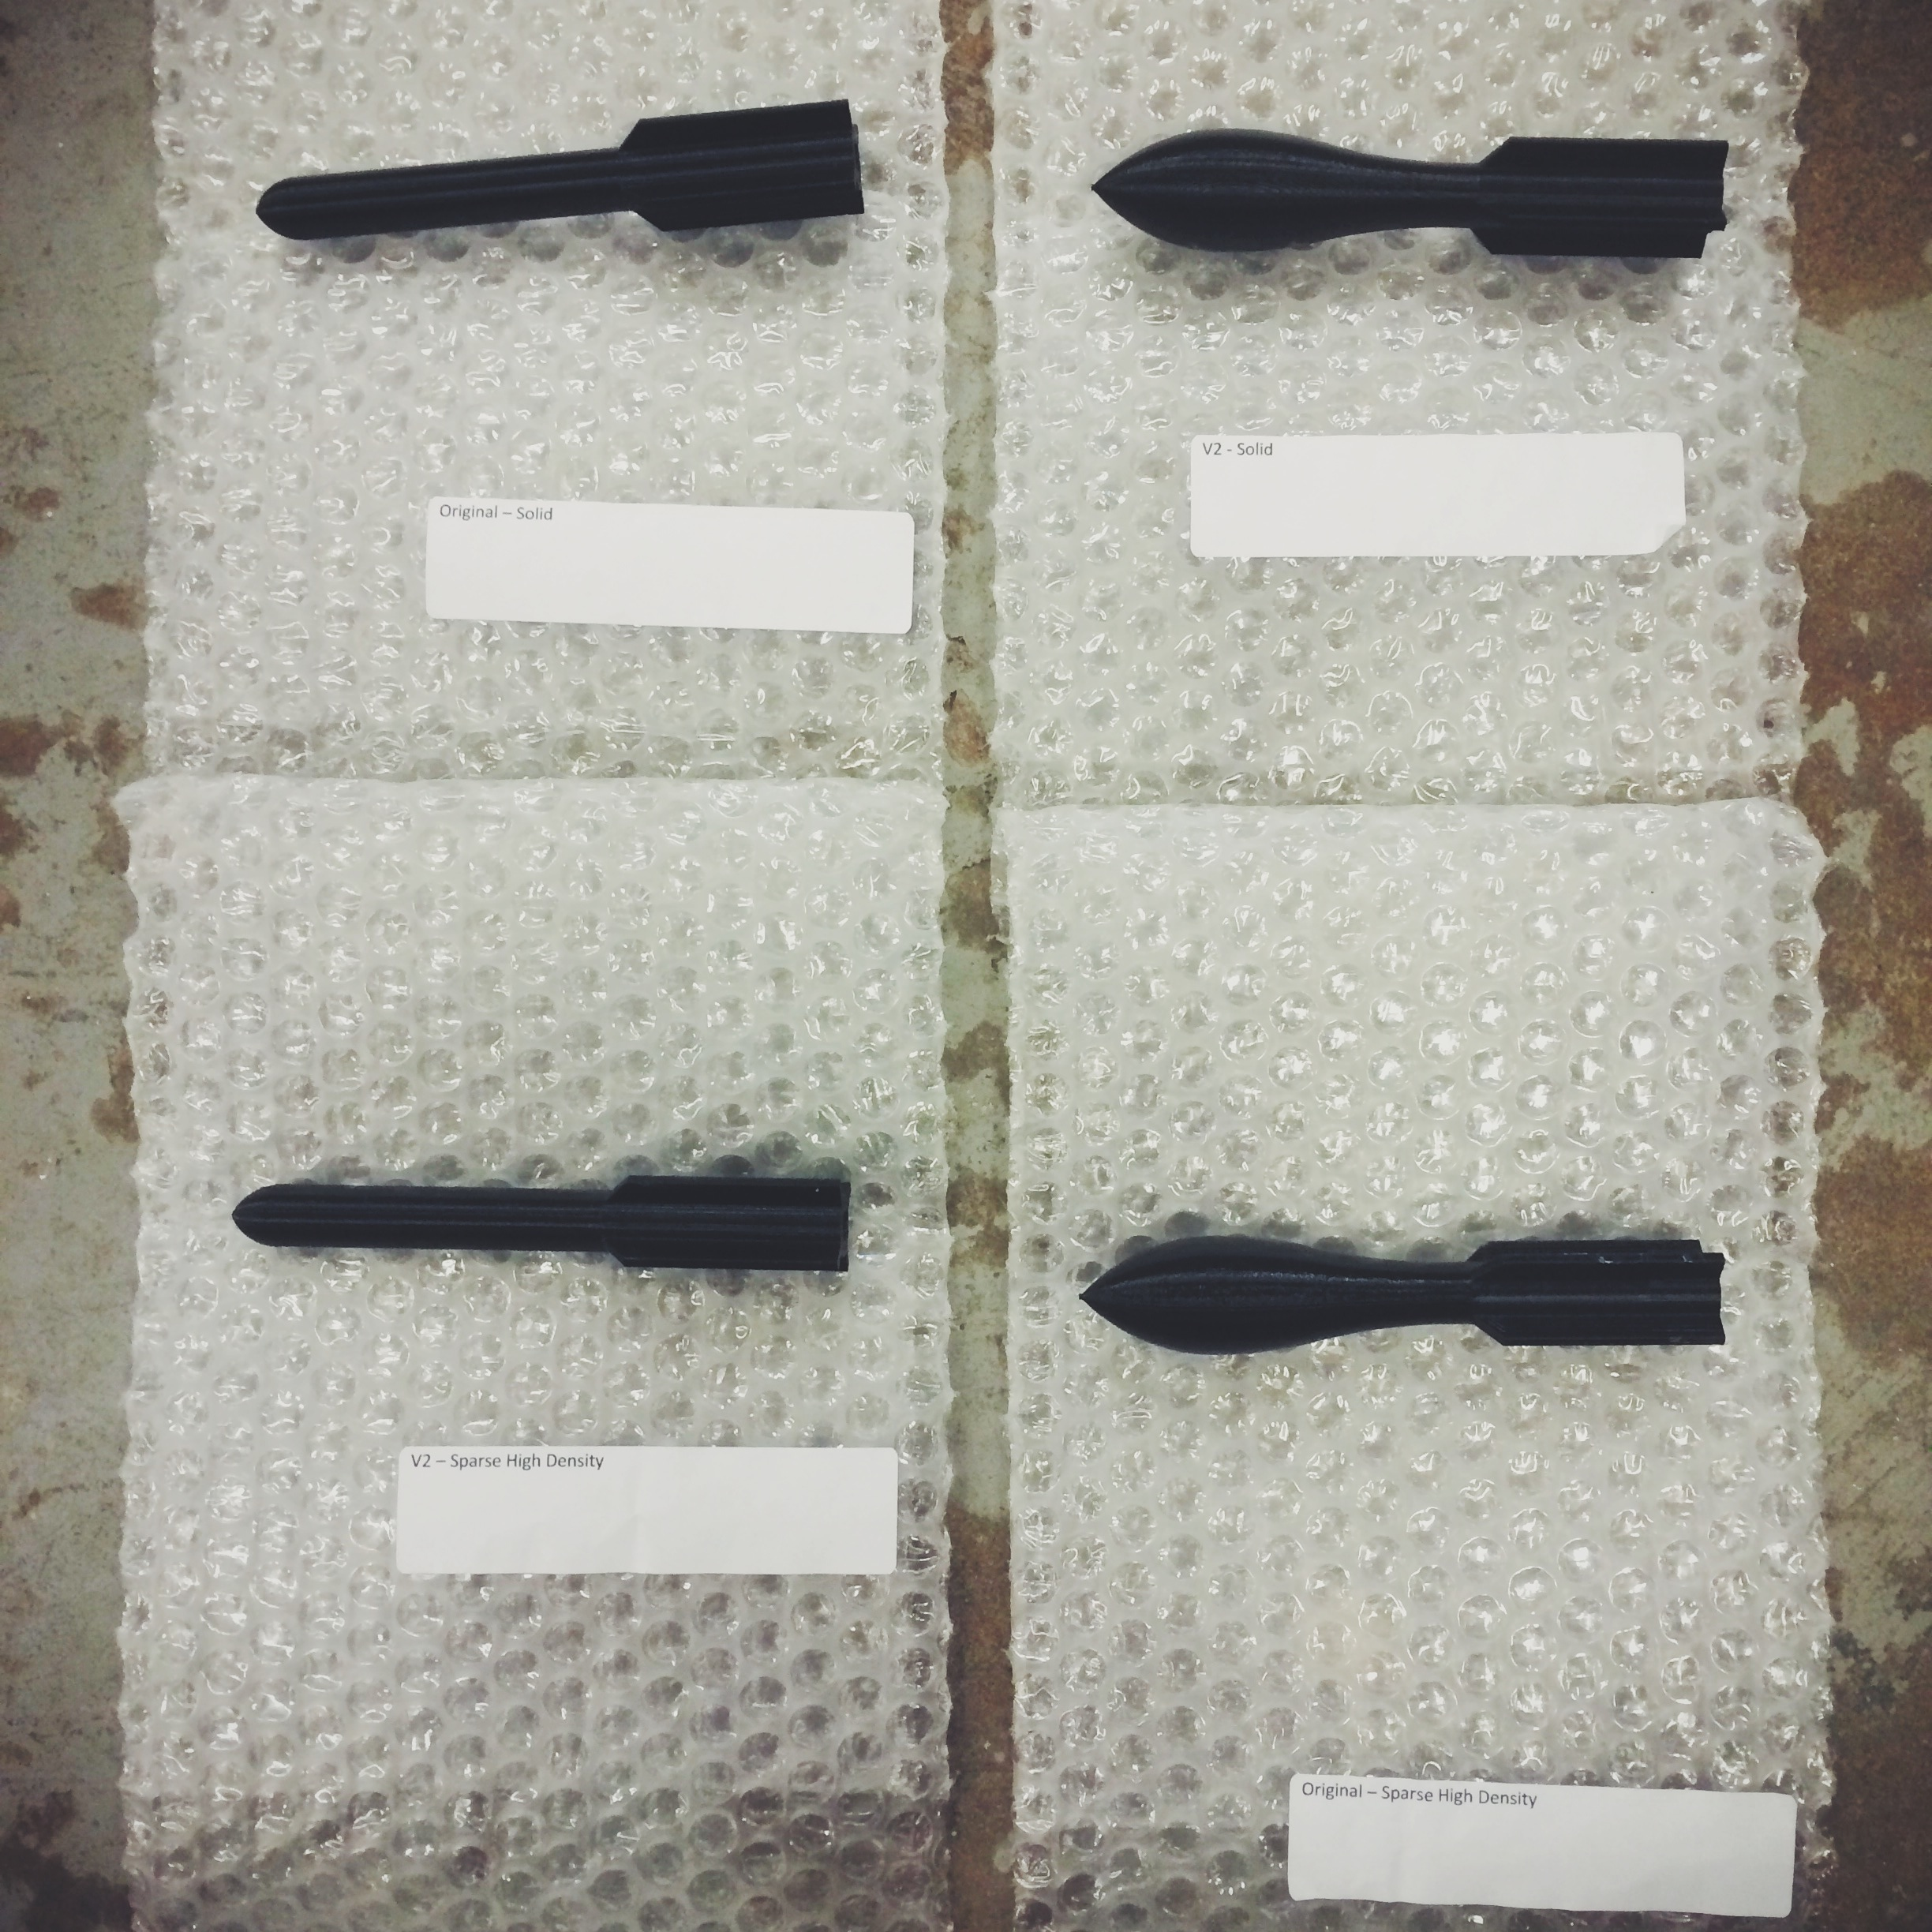
\includegraphics[height=4in]{media/torpedoes}
		\caption{Projectiles}
		\label{torpedo}
	\end{figure}

	The projectiles were printed in varying shapes and densities on the Fortus 360 to allow for testing and analysis of the different hydrodynamic and buoyancy properties.

	\begin{figure}[H]
		\centering
		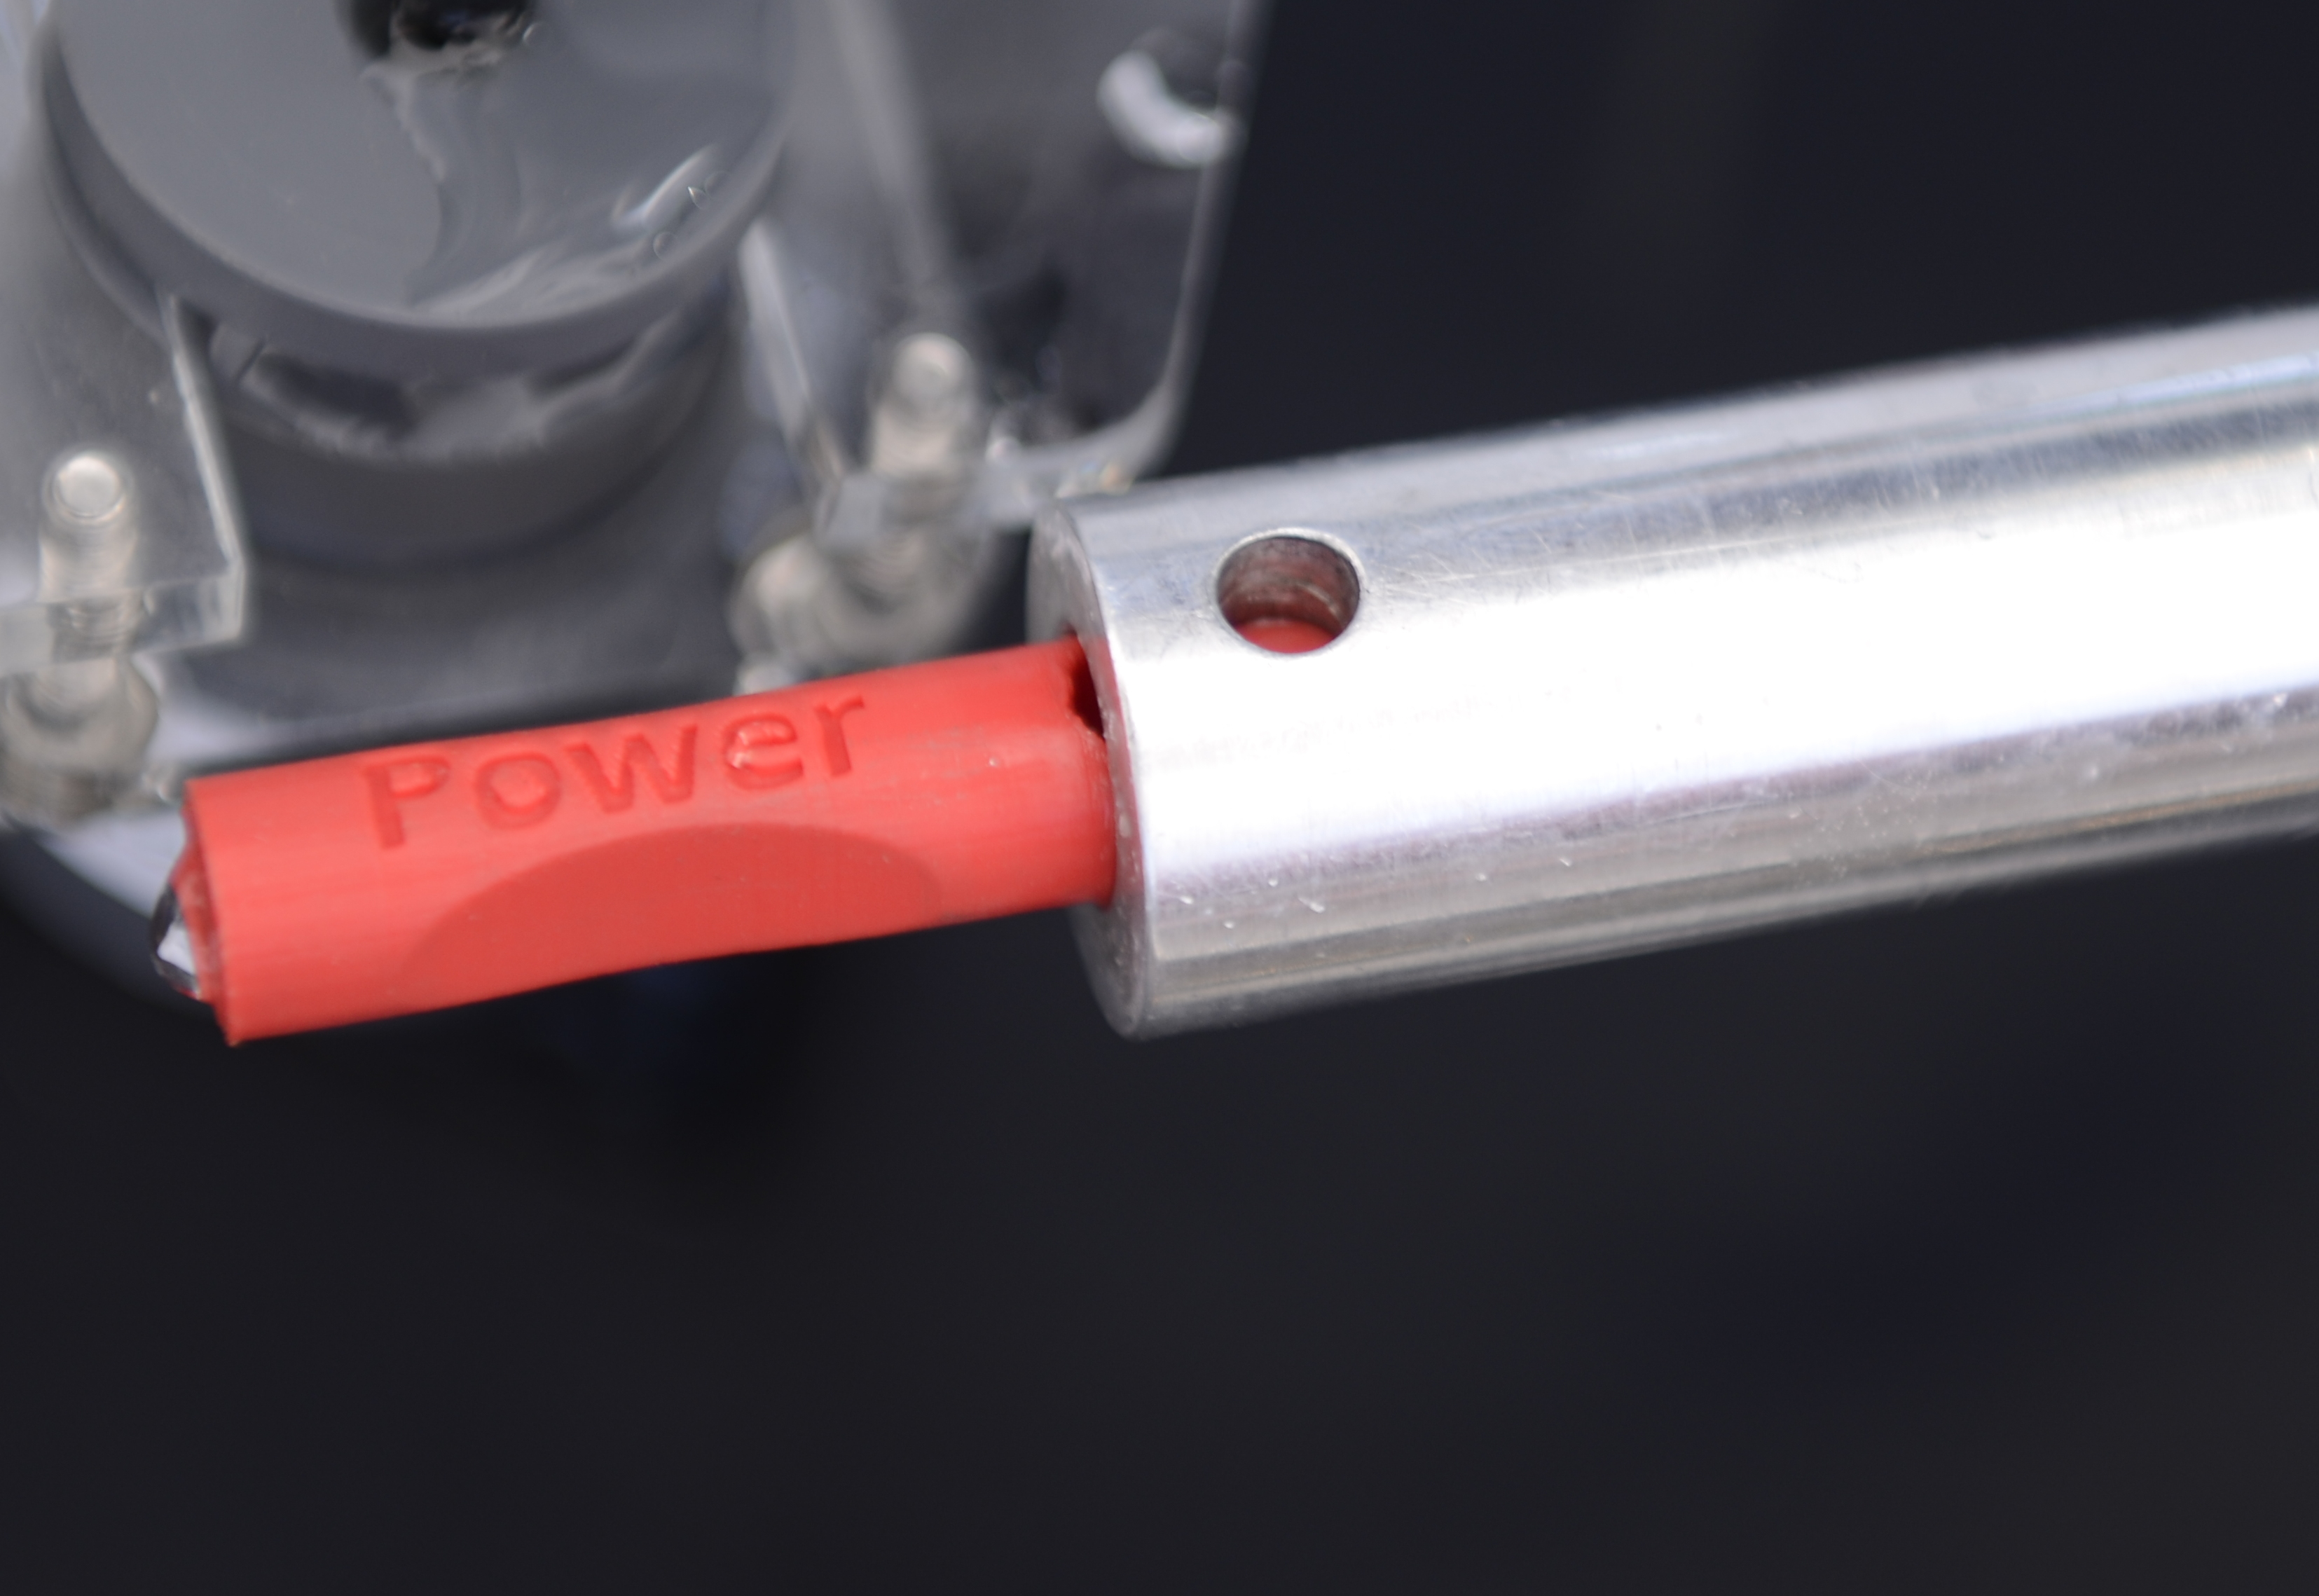
\includegraphics[height=4in]{media/kill_switch}
		\caption{Power switch}
		\label{torpedo}
	\end{figure}

	The power switch to the AUV was printed on a Makerbot Replicator 2X to act as a push button modification to an existing waterproof switch.  It was designed to fit inside the switch's chamber to depress a button, while another hole aligned with a pin, and finger grips afford its insertion.  A ring at the base of the button (hidden inside the chamber) keeps the piece from falling out.

\clearpage

% ENCLOSURE
	\section{Electronics Enclosure}
		\paragraph{Project:} Wearable Mixed-Signal Sensor Circuit for the McGill University \href{http://www.ece.mcgill.ca/~vchoda/Research.htm}{Sensor Microsystems Laboratory}
		\paragraph{Goal:} Enclose a small sensor circuit board with a hermetic seal and diaphragm to allow the measurement of pressure change under changing loads
		\paragraph{Description:} In order to pitch the device (sensor circuit board) to a potential client, a prototype of an enclosure was needed, with enough fidelity to sell the client on the functionality of the product.  The project was given to me on very short notice over a weekend, so was completed in one day.

	\begin{figure}[H]
		\centering
		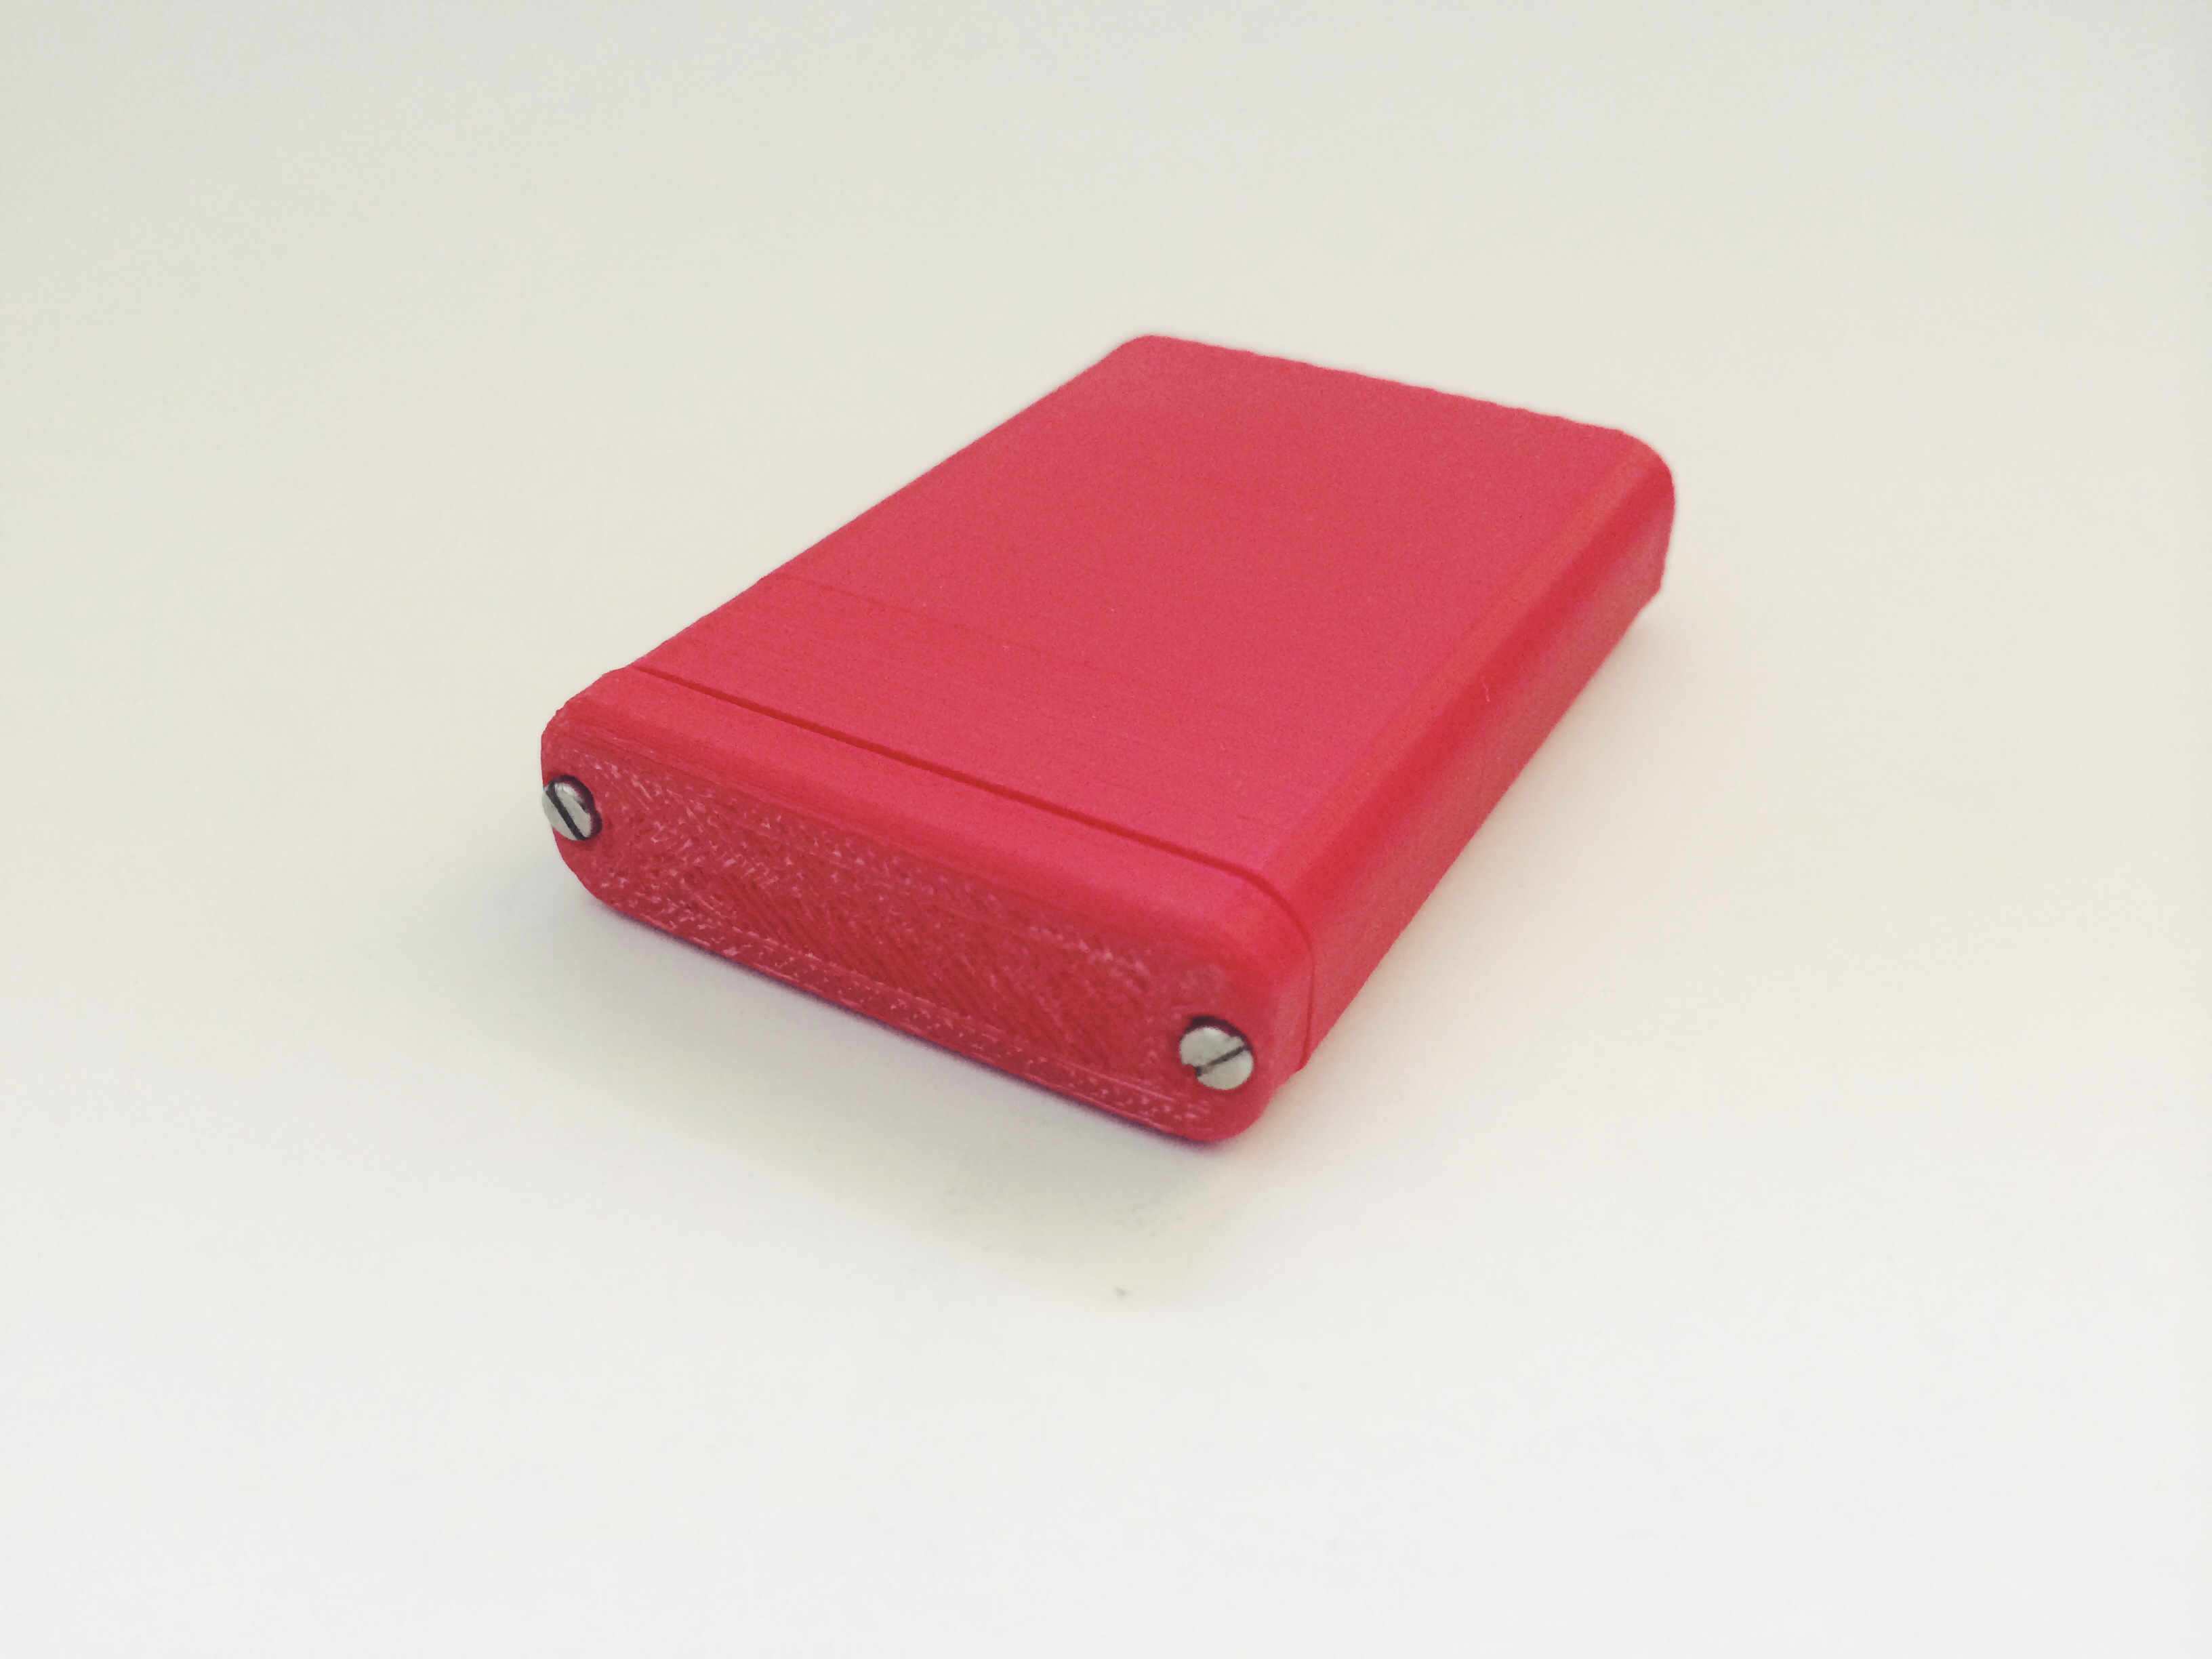
\includegraphics[height=4in]{media/enclosure_closed}
		\caption{Electronics enclosure sealed}
		\label{enclosure_sealed}
	\end{figure}

	The 3D printed prototype was designed to encapsulate a small circuit board and connected battery, with a hermetic o-ring seal, and fastened with two screws.  It was printed on a Makerbot Replicator 2X in one iteration.

	\begin{figure}[H]
		\centering
		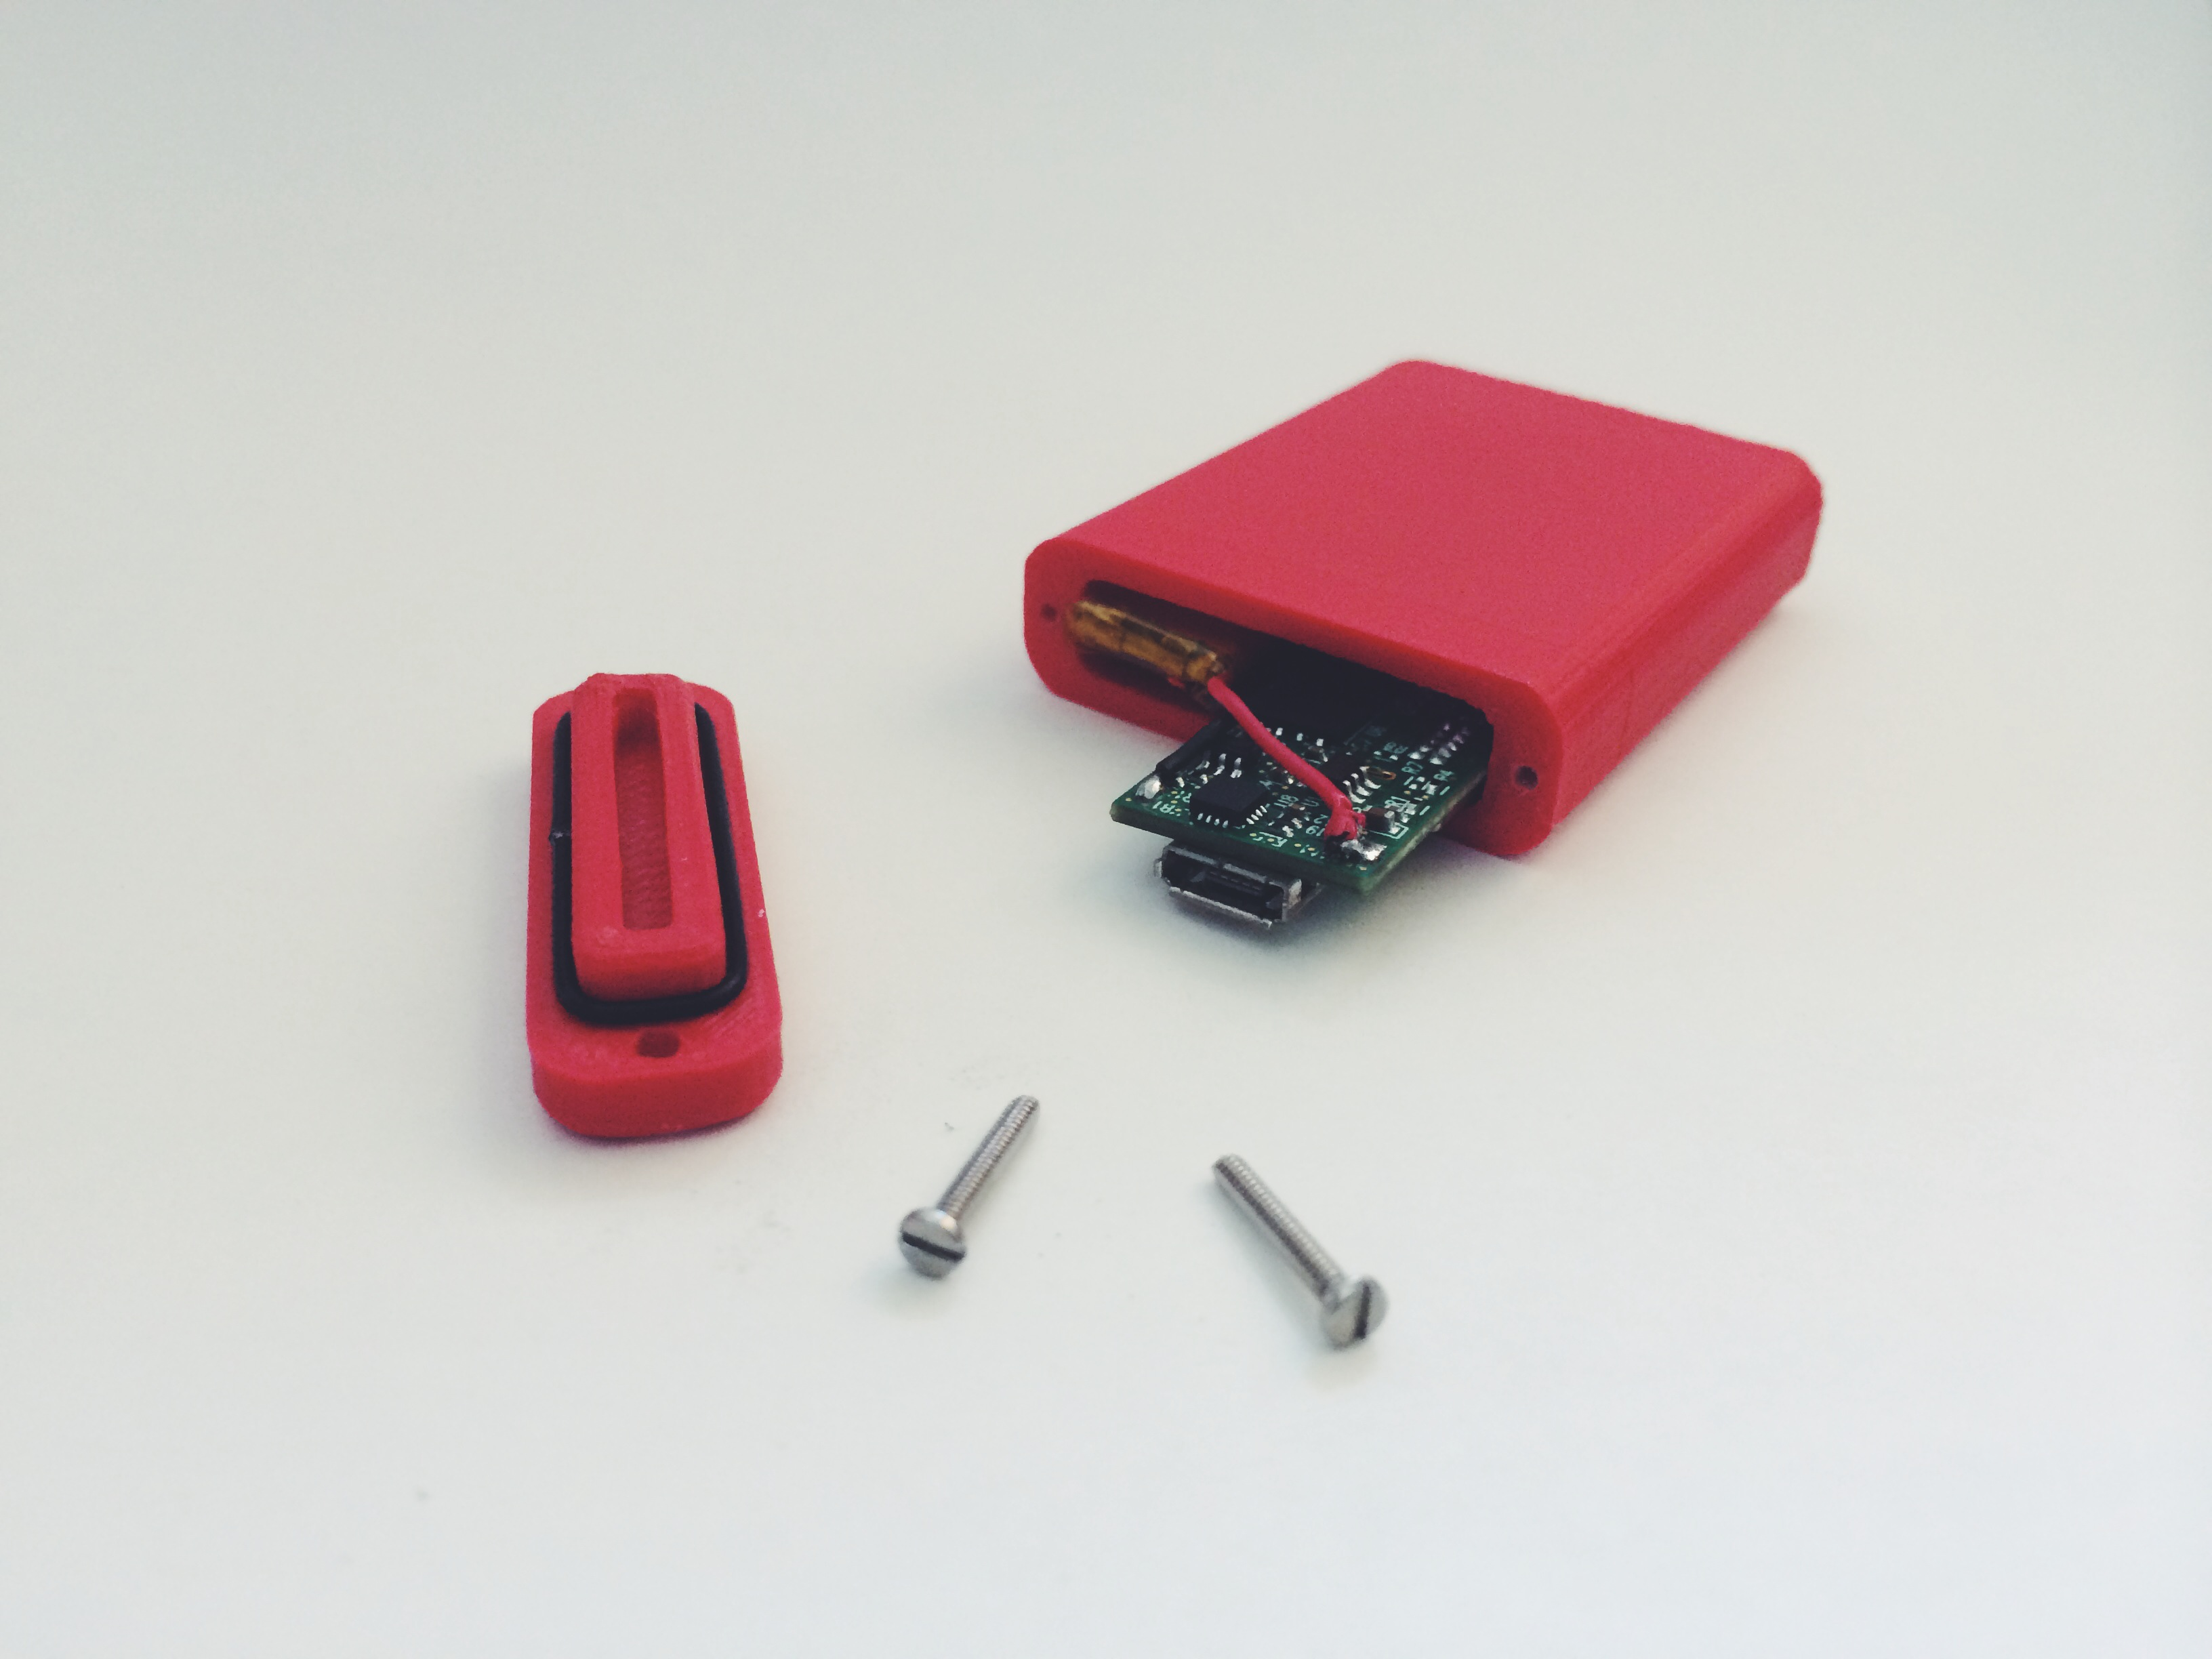
\includegraphics[height=4in]{media/enclosure_open}
		\caption{Electronics enclosure open}
		\label{enclosure_open}
	\end{figure}

	The enclosure is a very simple container and cap design, but one wall of the container is made thin (1.0mm thick) to create a flexible membrane that deforms under load, such that the pressure sensor inside can measure the change.


\end{document}